\documentclass[9pt,dvipsnames]{beamer}
\usepackage[T1]{fontenc}
\usepackage{libertinus}
\usepackage{amsmath}
\usepackage[most]{tcolorbox}
\usepackage{graphicx}

\usepackage{hyperref}

\usepackage{xcolor}  
\newcommand{\cb}[1]{{\color{CadetBlue}#1}}

\setlength{\parskip}{0.5em}
\usetheme{Berkeley}
\setbeamertemplate{navigation symbols}{}


\title{CSE574 Introduction to Machine Learning}
\subtitle{Support Vector Machine}
\author{Jue Guo}
\institute{University at Buffalo}
\date{\today}

\begin{document}
\begin{frame}
	\titlepage
\end{frame}

\begin{frame}
	This section is an adaptation of Andrew Ng's Machine Learning Course on SVM.
\end{frame}

\begin{frame}
	\frametitle{Outline}
	\tableofcontents
\end{frame}



\section{Alternative View of Logistic Regression}
\begin{frame}{Alternative View of Logistic Regression}
	\begin{columns}
		\column{0.5\textwidth}
		A quick review: $h_\theta(x)=\frac{1}{1+e^{-\theta^T x}}$
		\begin{itemize}
			\item if \(y=1\), we want $h_\theta(x) \approx 1$, $\theta^T x \gg 0$
			\item if \(y=0\), we want \(h_\theta(x) \approx 0\), $\theta^T x \ll 0$
		\end{itemize}
		\column{0.5\textwidth}
		\begin{figure}
			\centering
			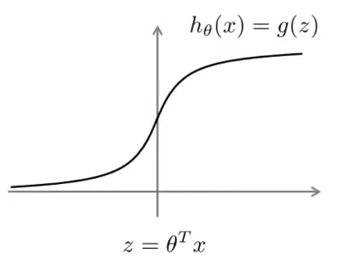
\includegraphics[width=0.9\textwidth]{imgs/svm_1.png}
		\end{figure}

	\end{columns}
	The cost of a single example:

	\begin{align*}
		  & -\left(y \log h_\theta(x)+(1-y) \log \left(1-h_\theta(x)\right)\right)                    \\
		= & -y \log \frac{1}{1+e^{-\theta^T x}}-(1-y) \log \left(1-\frac{1}{1+e^{-\theta^T x}}\right)
	\end{align*}
\end{frame}

\begin{frame}
	\[
		-y \log \frac{1}{1+e^{-\theta^T x}}-(1-y) \log \left(1-\frac{1}{1+e^{-\theta^T x}}\right)
	\]
	\begin{columns}
		\column{0.5\textwidth}
		if \(y=1\) (want $\theta^T x \gg 0$)
		\begin{figure}
			\centering
			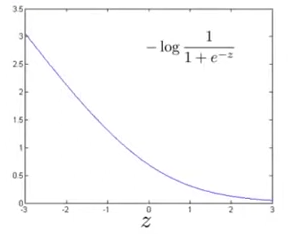
\includegraphics[width=0.7\textwidth]{imgs/svm_2.png}
		\end{figure}
		\column{0.5\textwidth}
		if \(y=0\) (want $\theta^T x \ll 0$)
		\begin{figure}
			\centering
			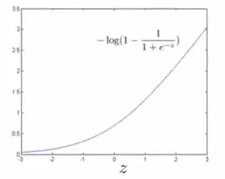
\includegraphics[width=0.7\textwidth]{imgs/svm_3.png}
		\end{figure}
	\end{columns}
\end{frame}

\section{Support Vector Machine}
\begin{frame}{Support Vector Machine}
	\textbf{Cost Function of Logistic Regression}
	\begin{align*}
		\min _\theta \frac{1}{m}\Bigg[ & \sum_{i=1}^m y^{(i)}\left(-\log h_\theta\left(x^{(i)}\right)\right)\\
		                               & + \left(1-y^{(i)}\right)\left(-\log \left(1-h_\theta\left(x^{(i)}\right)\right)\right)\Bigg] \\
		                               & + \frac{\lambda}{2 m} \sum_{j=1}^n \theta_j^2
	\end{align*}
	\textbf{Cost Function of Support Vector Machine}
	$$
		\min _\theta C \sum_{i=1}^m\left[y^{(i)} \operatorname{cost}_1\left(\theta^T x^{(i)}\right)+\left(1-y^{(i)}\right) \operatorname{cost}_0\left(\theta^T x^{(i)}\right)\right]+\frac{1}{2} \sum_{i=1}^n \theta_j^2
	$$
\end{frame}

\subsection{Large Margin Intuition}
\begin{frame}{Large Margin Intuition}
	\textbf{Support Vector Machine}
	$$
		\min _\theta C \sum_{i=1}^m\left[y^{(i)} \operatorname{cost}_1\left(\theta^T x^{(i)}\right)+\left(1-y^{(i)}\right) \operatorname{cost}_0\left(\theta^T x^{(i)}\right)\right]+\frac{1}{2} \sum_{i=1}^n \theta_j^2
	$$
	\begin{columns}
		\column{0.5\textwidth}
		\begin{figure}
			\centering
			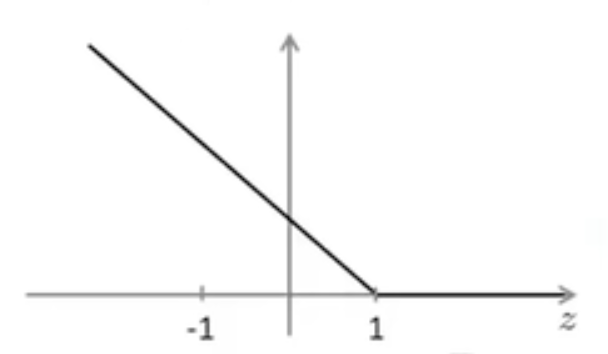
\includegraphics[width=\textwidth]{imgs/svm_4.png}
		\end{figure}
		If \(y=1\), we want \(\theta^{T} x \geq 1\) (not just \(\left.\geq 0\right)\)
		
		\column{0.5\textwidth}
		\begin{figure}
			\centering
			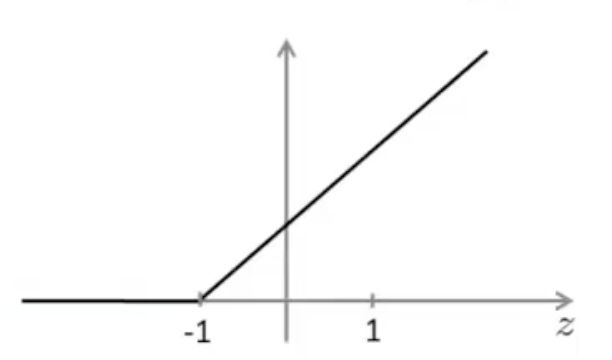
\includegraphics[width=\textwidth]{imgs/svm_5.png}
		\end{figure}
		If \(y=0\), we want \(\theta^{T} x \leq-1\) (not just \(\left.<0\right)\)
	\end{columns}
\end{frame}

\begin{frame}{A very large \(C\)}
	\textbf{Support Vector Machine}
	$$
	\min _\theta C \sum_{i=1}^m\left[y^{(i)} \operatorname{cost}_1\left(\theta^T x^{(i)}\right)+\left(1-y^{(i)}\right) \operatorname{cost}_0\left(\theta^T x^{(i)}\right)\right]+\frac{1}{2} \sum_{i=1}^n \theta_j^2
	$$
	Given that \(C\) is a very large value, we want that the first term to be \(0\). Let's try to understand the optimization problem in the context of what would it take to make this first term in the objective equal to \(0\). 
	\vspace{0.3cm}
	\begin{columns}
		\column{0.5\textwidth}
		Whenever \(y^{(i)}=1\), \(\theta^{\top} x^{(i)} \geqslant 1\); 
		\column{0.5\textwidth}
		Whenever \(y^{(i)}=0\), \(\theta^{\top} x^{(i)} \leqslant-1\)
	\end{columns}
	
	Now, the optimization problem can be written as: 
	\begin{equation*}
		\begin{aligned}
			& \text{min} C\cdot 0 + \frac{1}{2}\sum_{i=1}^n \theta_j^2 \\
			\text{s.t.  } &  \theta^{\top} x^{(i)} \geqslant 1 \quad \text { if } y^{(i)}=1 \\
			& \theta^{T} x^{(i)} \leqslant-1 \quad \text {if } y^{(i)}=0
		\end{aligned}
	\end{equation*}
\end{frame}

\begin{frame}
	\textbf{SVM Decision Boundary: Linearly separable case}
\begin{figure}
	\centering
	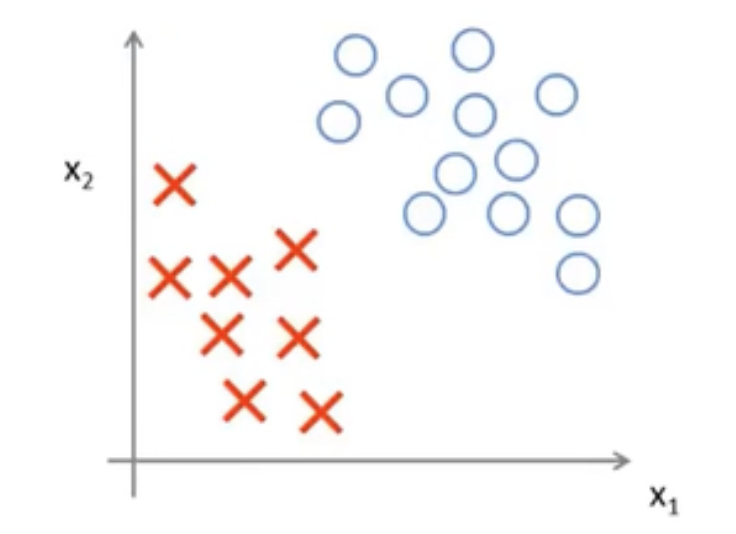
\includegraphics[width=0.4\linewidth]{imgs/svm_6}
	\caption{Linearly Separable Case}
	\label{fig:svm6}
\end{figure}
\end{frame}

\begin{frame}
	\textbf{Large margin classifier in presence of outliers}
	\begin{figure}
		\centering
		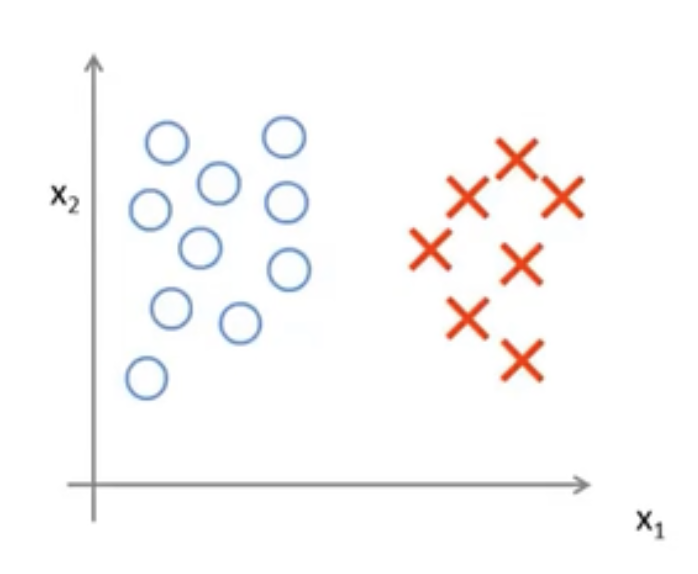
\includegraphics[width=0.4\linewidth]{imgs/svm_7}
		\label{fig:svm7}
	\end{figure}
\end{frame}

\subsection{The Mathematics behind Large Margin Classification}
\begin{frame}{The Mathematics behind Large Margin Classification}
	\textbf{Vector Inner Product}
\end{frame}
\begin{frame}
	\begin{center}
		\Huge Questions?
	\end{center}
\end{frame}
\end{document}